\section{Evaluation}
To evaluate the impact flat combining has on the global data structures, we ran a series of experiments to test the raw performance of the data structures themselves under different workloads, and then measure their impact on performance of two simple graph benchmarks.

Experiments were run on a cluster of AMD Interlagos processors. Nodes have 32 2.1-GHz cores in two sockets, 64GB of memory, and 40Gb Mellanox ConnectX-2 InfiniBand network cards, connected via a QLogic InfiniBand switch.

\subsection{Data Structure Throughput}
First we measured the raw performance of the global data structures on extremely simple throughput workloads. In each experiment, a Grappa parallel loop spawns an equal number of tasks on all cores. Each task randomly chooses an operation based on the predetermined ``operation mix,'' selecting either a push or pop for the Stack and Queue, or an insert or lookup for the Set and Map.

\paragraph{Queue and Stack}
\begin{figure}[t]
  \centering
  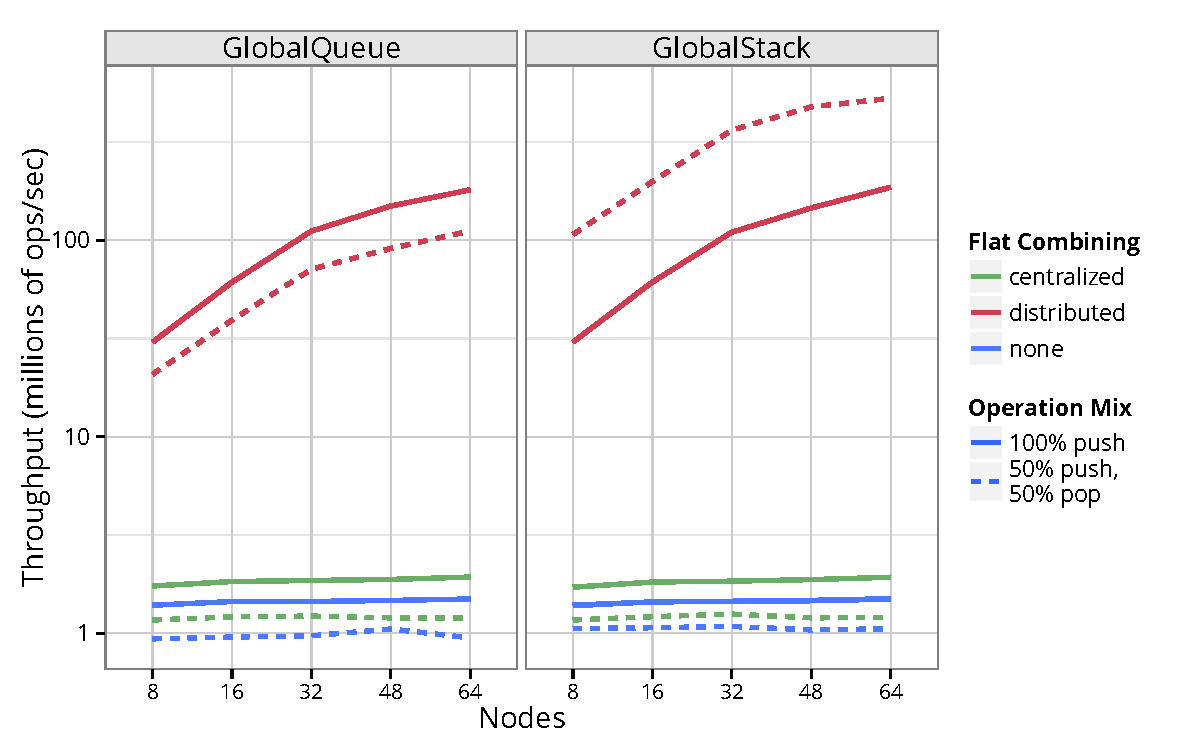
\includegraphics[width=0.5\textwidth]{data/plots/vector_perf.pdf}
  \caption{\emph{Queue and Stack performance.}
    Results are shown on a log scale for a throughput workload performing 256 million operations with 2048 workers per core and 16 cores per node. Local flat combining improves throughput by at least an order of magnitude and allows performance to scale. Matching pushes and pops enables the stack to perform even better on a mixed workload.
  }
  \label{fig:vector}
\end{figure}

\begin{figure}[t]
  \centering
  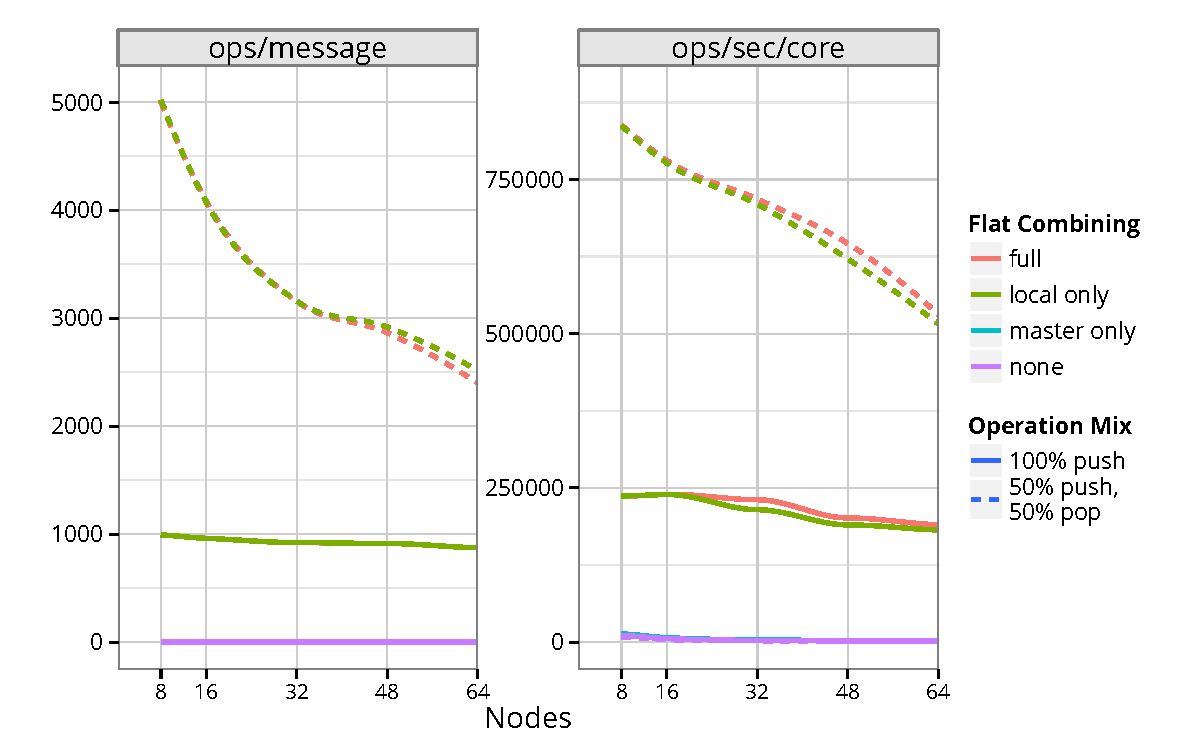
\includegraphics[width=0.5\textwidth]{data/plots/stack_stats.pdf}
  \caption{\emph{GlobalStack Statistics.}
    Measured number of combined messages sent by the Stack with a fixed combining buffer of 1024 elements.
    Matched pushes and pops result in ops/message being greater than the buffer size.
  }
  \label{fig:stack_stats}
\end{figure}

Figure~\ref{fig:vector} shows the results of the throughput experiments for the global Stack and Queue. Results are shown with flat combining completely disabled, only combining at the master core (``centralized''), and combining locally (``distributed'').

Despite Grappa's automatic aggregation, without combining, both the stack and queue completely fail to scale because all workers' updates must serialize.
Though centralized combining alleviates some of the serialization, its benefit is limited because all synchronization must still be performed on one core. However, with local flat combining, synchronization is able to be done mostly in parallel, with less-frequent bulk synchronization at the master.

On the mixed workload, the stack is able to do matching locally, allowing it to reduce the amount of communication drastically, greatly improving its performance on the mixed workload. Figure~\ref{fig:stack_stats} corroborates this, showing that the amount of combining that occurs directly correlates with the observed throughput.

We also experimented with performing both forms of combining together; however, combining at the master did not affect performance significantly. This was somewhat surprising as combined updates still force others to wait. However, with both levels of combining enabled, relatively few requests are combined at the master--for the all-push workload, on the order of a thousand, and for the mixed workload on the stack, the average is less than 20.

The queue benefits in the same way from reducing synchronization and batching, and its all-push workload performs identically to the stack's.
However, the queue is unable to do matching locally, and in fact, the mixed workload performs worse because the current implementation serializes combined pushes and combined pops. This restriction could be lifted with more careful synchronization at the master core.

\paragraph{HashSet and HashMap}
\begin{figure}[t]
  \centering
  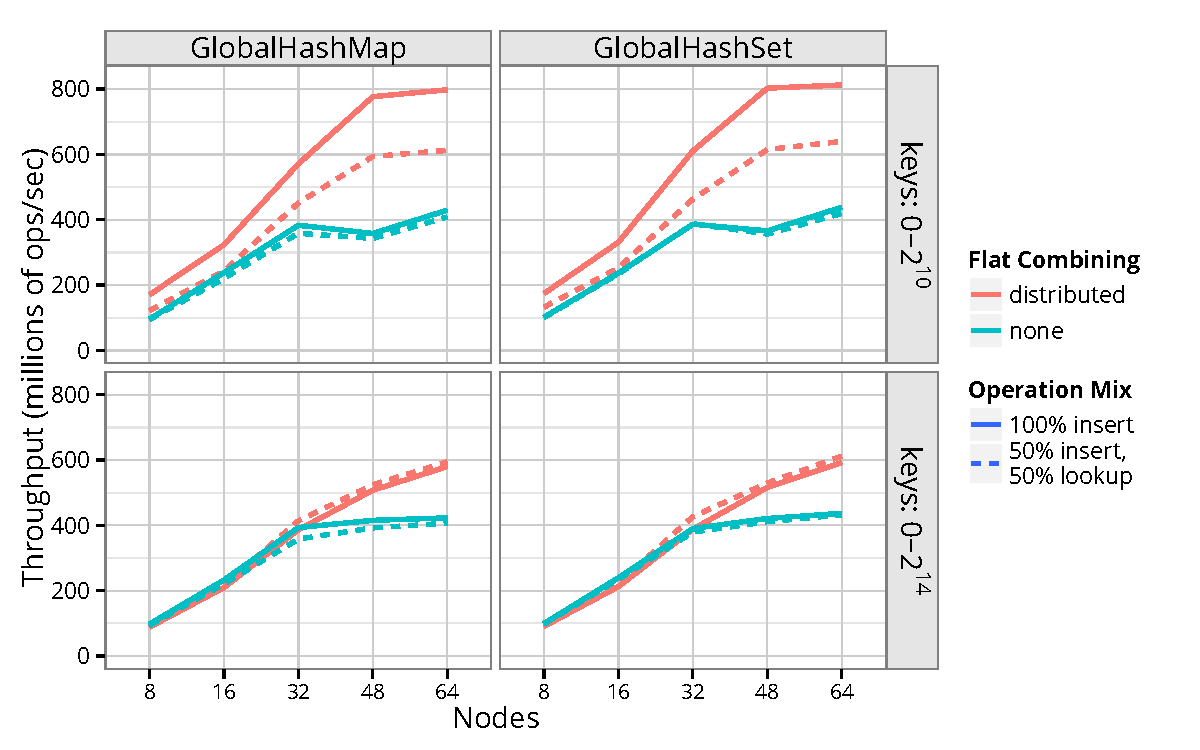
\includegraphics[width=0.5\textwidth]{data/plots/hash_perf.pdf}
  \caption{\emph{GlobalHashSet and GlobalHashMap.}
    Results are shown for a throughput workload inserting and looking up 256 million random keys in a particular range into a global hash with the same number of cells, with 2048 workers per core and 16 cores per node.
  }
  \label{fig:hash_perf}
\end{figure}

% Without combining, performance scales out to 32 nodes because synchronization is distributed over hash cells, but drops off as the number of destinations increases.
Figure~\ref{fig:hash_perf} shows the throughput results for the Set and Map.
Both data structures synchronize at each hash cell, which allows them to scale fairly well even without combining. However, after 32 nodes, scaling drops off significantly due to the increased number of destinations.
Combining allows duplicate inserts and lookups to be eliminated, so performs better the smaller the key range. This reduction in message traffic allows scaling to continue out to 64 nodes.

\subsection{Application Kernel Performance}
The original goal was to have scalable global data structures in the Grappa library that could be used in applications. Generic implementations of data structures are often insufficient for scaling, so HPC applications often implement their own customized versions. However, this forces each application to carefully reason about the ways in which the structures will be accessed, and often relies on relaxing consistency.
The Grappa data structures are synchronized to provide the most general use and match the expectations of programmers and algorithms.
In these evaluations, we compare the flat-combining structures against tuned, relaxed-consistency versions.

\paragraph{Breadth-First Search}
\begin{figure}[t]
  \centering
  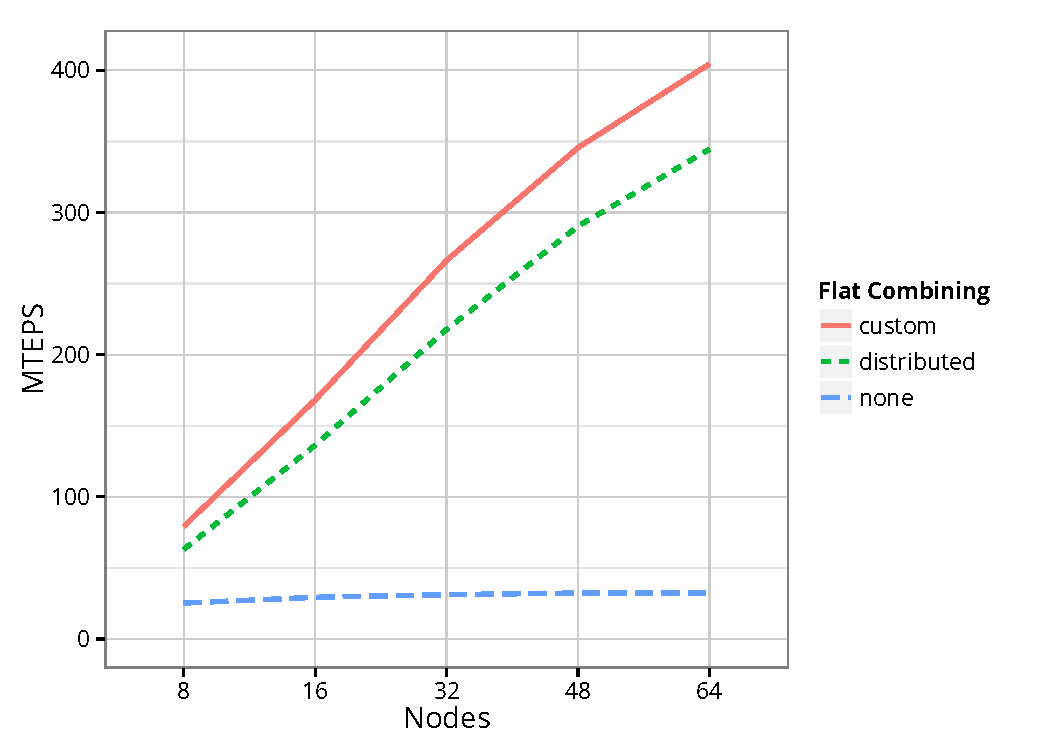
\includegraphics[width=0.5\textwidth]{data/plots/bfs_perf.pdf}
  \caption{\emph{BFS} on a Graph500-spec graph of scale 26 (64 million vertices, 1 billion edges), with the direction-optimizing BFS algorithm. Performance is measured in millions of Traversed Edges Per Second (MTEPS).}
  \label{fig:bfs_perf}
\end{figure}
The first application kernel is the Graph500 Breadth-First-Search (BFS) benchmark~\cite{graph500list}. This benchmark does a search starting from a random vertex in a synthetic graph and builds a search tree of parent vertices for each vertex traversed during the search. While this is a relatively simple problem, it exercises the random-access throughput of a system as well as being a primitive in many other graph algorithms. The BFS algorithm contains a global queue which represents the frontier of vertices to be visited in each level.
Our implementation employs the direction-optimizing algorithm by Beamer et al.~\cite{Beamer:Graph500} which performs particularly well for the scale-free RMAT graphs generated by the benchmark.
The frontier queue in BFS is amenable to further optimization to take advantage of the fact that the algorithm does pushes and pops in separate phases, allowing consistency to be relaxed.
We compare our implementation of BFS using the flat-combined global queue described above with a highly tuned Grappa implementation that uses a custom asynchronous queue.

Figure~\ref{fig:bfs_perf} shows the results of scaling the BFS kernel up to 64 nodes. The simple queue implementation without flat combining is completely unscalable. However, the flat combining queue tracks the tuned version. This illustrates that providing a safe, synchronized data structure for initially developing algorithms for PGAS is possible without sacrificing scaling.
% , while further optimizations can be applied incrementally.

\paragraph{Connected Components}
\begin{figure}[t]
  \centering
  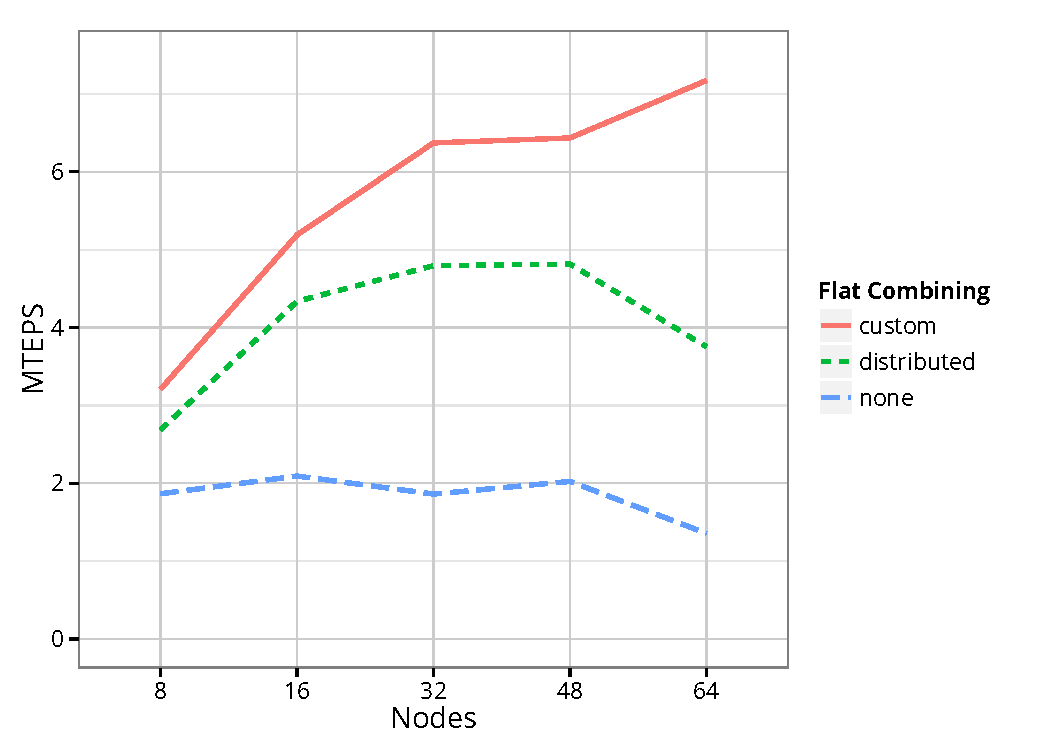
\includegraphics[width=0.5\textwidth]{data/plots/cc_perf.pdf}
  \caption{\emph{Connected Components} on the same scale 26 Graph500 graph. Performance is measured in MTEPS.}
  \label{fig:cc_perf}
\end{figure}
Connected Components (CC) is another simple graph analysis kernel that illustrates a different use of global data structures in irregular applications. We implement the three-phase CC algorithm~\cite{mtgl} which was designed for the massively parallel MTA-2 machine. In the first phase, parallel traversals attempt to claim vertices and label them.
Whenever two traversals encounter each other, an edge between the two roots is inserted in a set. After all edges have been traversed in this way, the set of edges forms a new, typically much smaller, graph. The second phase performs the classical Shiloach-Vishkin parallel algorithm~\cite{shiloach1982n} on this reduced graph, and the final phase propagates the component labels out to the full graph.
Creation of the reduced graph dominates the runtime of this algorithm, but includes many repeated inserts at the boundary between traversals, so is a prime target for the flat-combining Set.
As in BFS, further optimizations involving relaxation of consistency can be applied, in this case to the Set. Therefore, we compare our straightforward implementation using the generic Set with and without flat combining against a tuned asynchronous implementation.

The results in Figure~\ref{fig:cc_perf} show that none of these three scale well out to 64 nodes. However, performing combining does improve the performance over the uncombined case. The tuned version outperforms the synchronous version because it is able to build up most of the set locally on each core before merging them at the end of the first phase. An implementation that did not provide synchronized semantics could potentially relax consistency in a more general way, but this is left for future work.
